\chapter{INTRODUCTION}
\label{chap:intro}

The installed capacity of solar power in the US continues to grow as a
result of aging coal and natural gas power plants, lower costs,
state renewable portfolio standards, and efforts to decarbonize the
electrical grid.
As shown in \Cref{fig:solarinstall}, this growth has been steady since
2010 and shows no signs of abating.

\begin{figure}[htb]
  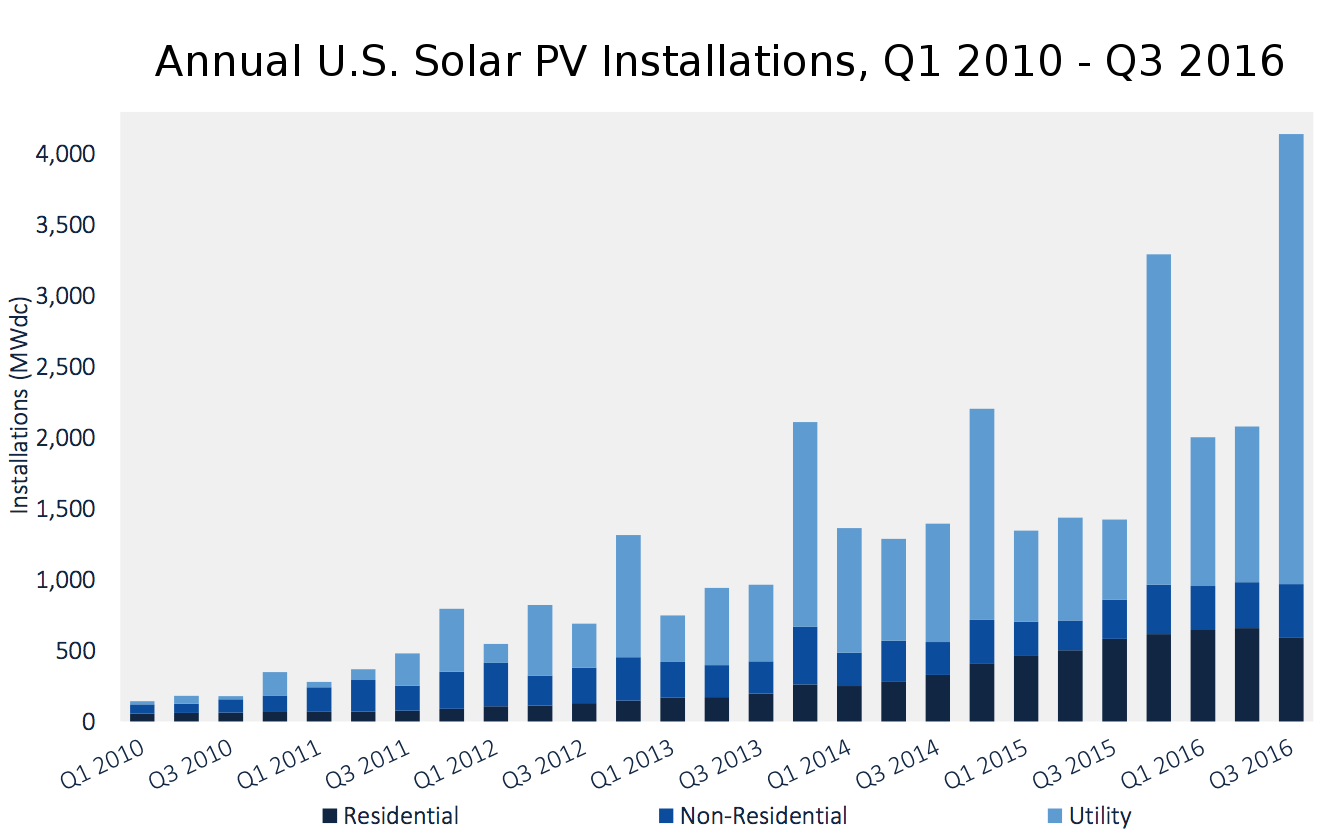
\includegraphics[width=\textwidth]{figs/solar_installations.png}
  \caption[Annual installations of solar PV in the US]{Annual
    installations of solar photovoltaic (PV) systems in the
    US. [Source:~\cite{GTM/SEIA2016}]}
\label{fig:solarinstall}
\end{figure}

Sunlight is the fuel that drives all solar power plants.
Unlike sources of fuel for conventional power generators like coal or
natural gas, the solar resource is highly variable due to the chaotic
nature of the weather.
This variability of the solar resource leads to uncertainty at the
electric utility and increases management costs \citep{Joskow2011}.
Forecasts help utilities manage the variability in a number of ways
\citep{Kleissl2013,Inman2013}, including the optimal dispatch of
battery storage \citep{Cormode2015}.
Improvements in forecasts further reduce costs
\citep{BrancucciMartinez-Anido2016}.
Ultimately, better forecasts increase the amount of solar power that
utilties can add to the grid.

An example of the variability that a 28 MW power plant experiences due
to clouds is shown in \cref{fig:variability_example}.
The power plant start producing power near sunrise, and reaches it's
peak power output of 28 MW in a few hours.
However, clouds begin moving over the plant in the afternoon causing
large fluctuations in the power.
Ramps (change in power per time) as large as 25 MW occur in a span of
5 minutes.
Utility companies need to constantly match the electrical generation
to the demand, which means the utility needs to be have generation
standing by that can provide the power as a cloud passes over the
plant and turn off quickly when the solar plant returns to normal
operation.


\begin{figure}[h]
\centering
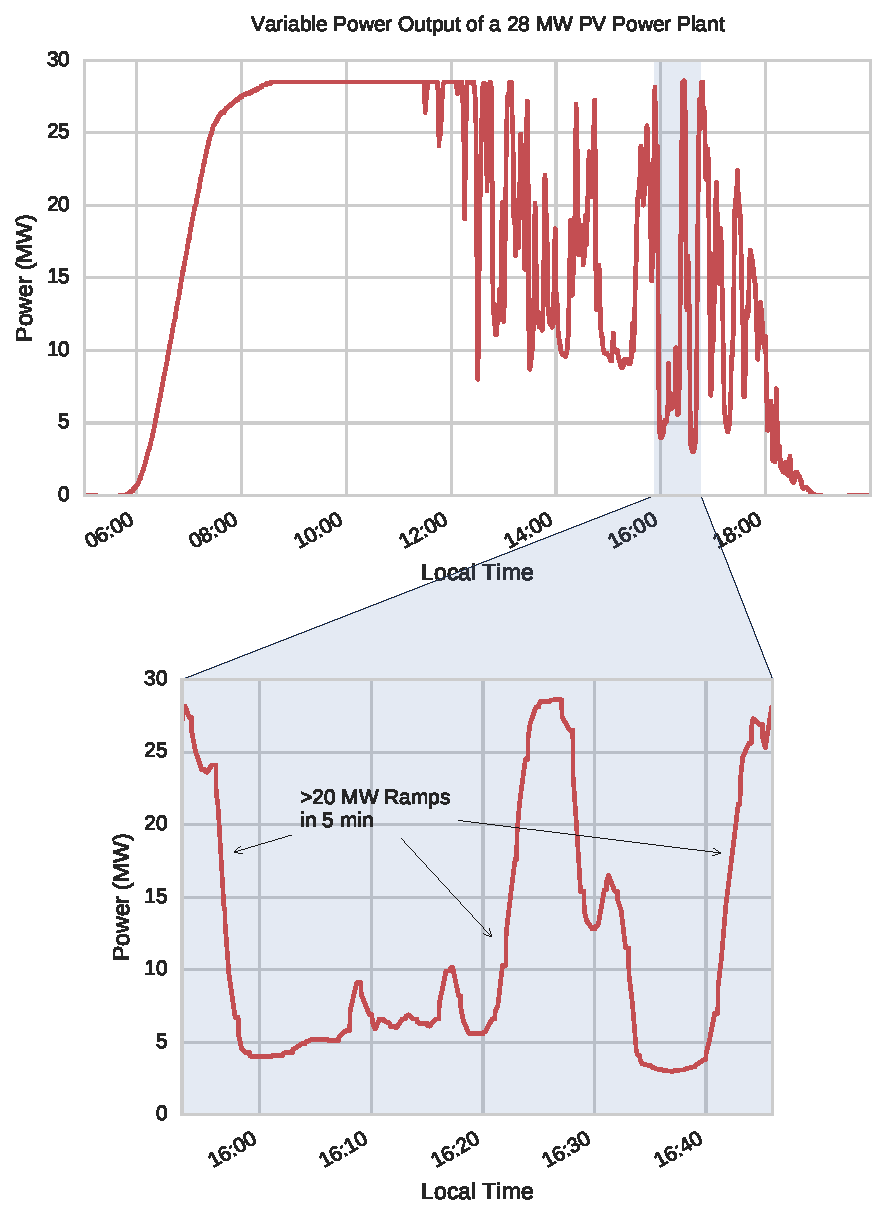
\includegraphics[width=.9\textwidth]{figs/avalon_ramps.pdf}
\caption[Variable power output of a 28 MW solar power plant]{
Power output of a 28 MW power plant near Tucson, AZ on a variable
day. Changes in power as large as 25 MW can occur in a span of only 5
minutes. This variability stresses the grid, but can be managed with
proper forecasting.}
\label{fig:variability_example}
\end{figure}

This dissertation will explore solar forecasting techniques to
mitigate this variability that incorporate data from a ground sensor
network.
First, the current state of solar power in the Southwest US and a
brief overview of general solar forecasting methods will be
discussed.
Then, a summary of the work in this dissertation will be provided
before diving into the details.

\section{State of Solar Power in the Southwest}

As of early 2017, members of the Southwest Variable Energy Resource
Initiative (SVERI) have a total of 1100 MW of installed solar capacity,
800 MW of installed wind capacity, and a peak load of 23 GW
\citep{sveri_website}.
Another roughly 1 GW of generation comes from distributed generation
(DG) solar systems that are installed on residential or commercial
rooftops.
Heatmaps showing the time of day load, wind generation, solar generation, and
wind and solar fraction of load for two years are shown in
\cref{fig:sveri_heatmap}.
Heatmaps for weather variables at the University of Arizona are shown
in \cref{fig:ua_heatmap} to correlate weather to, for example, the
abrupt decrease in load around 10/14 corresponding to the end of monsoon season.

\begin{figure}[p]
\centering
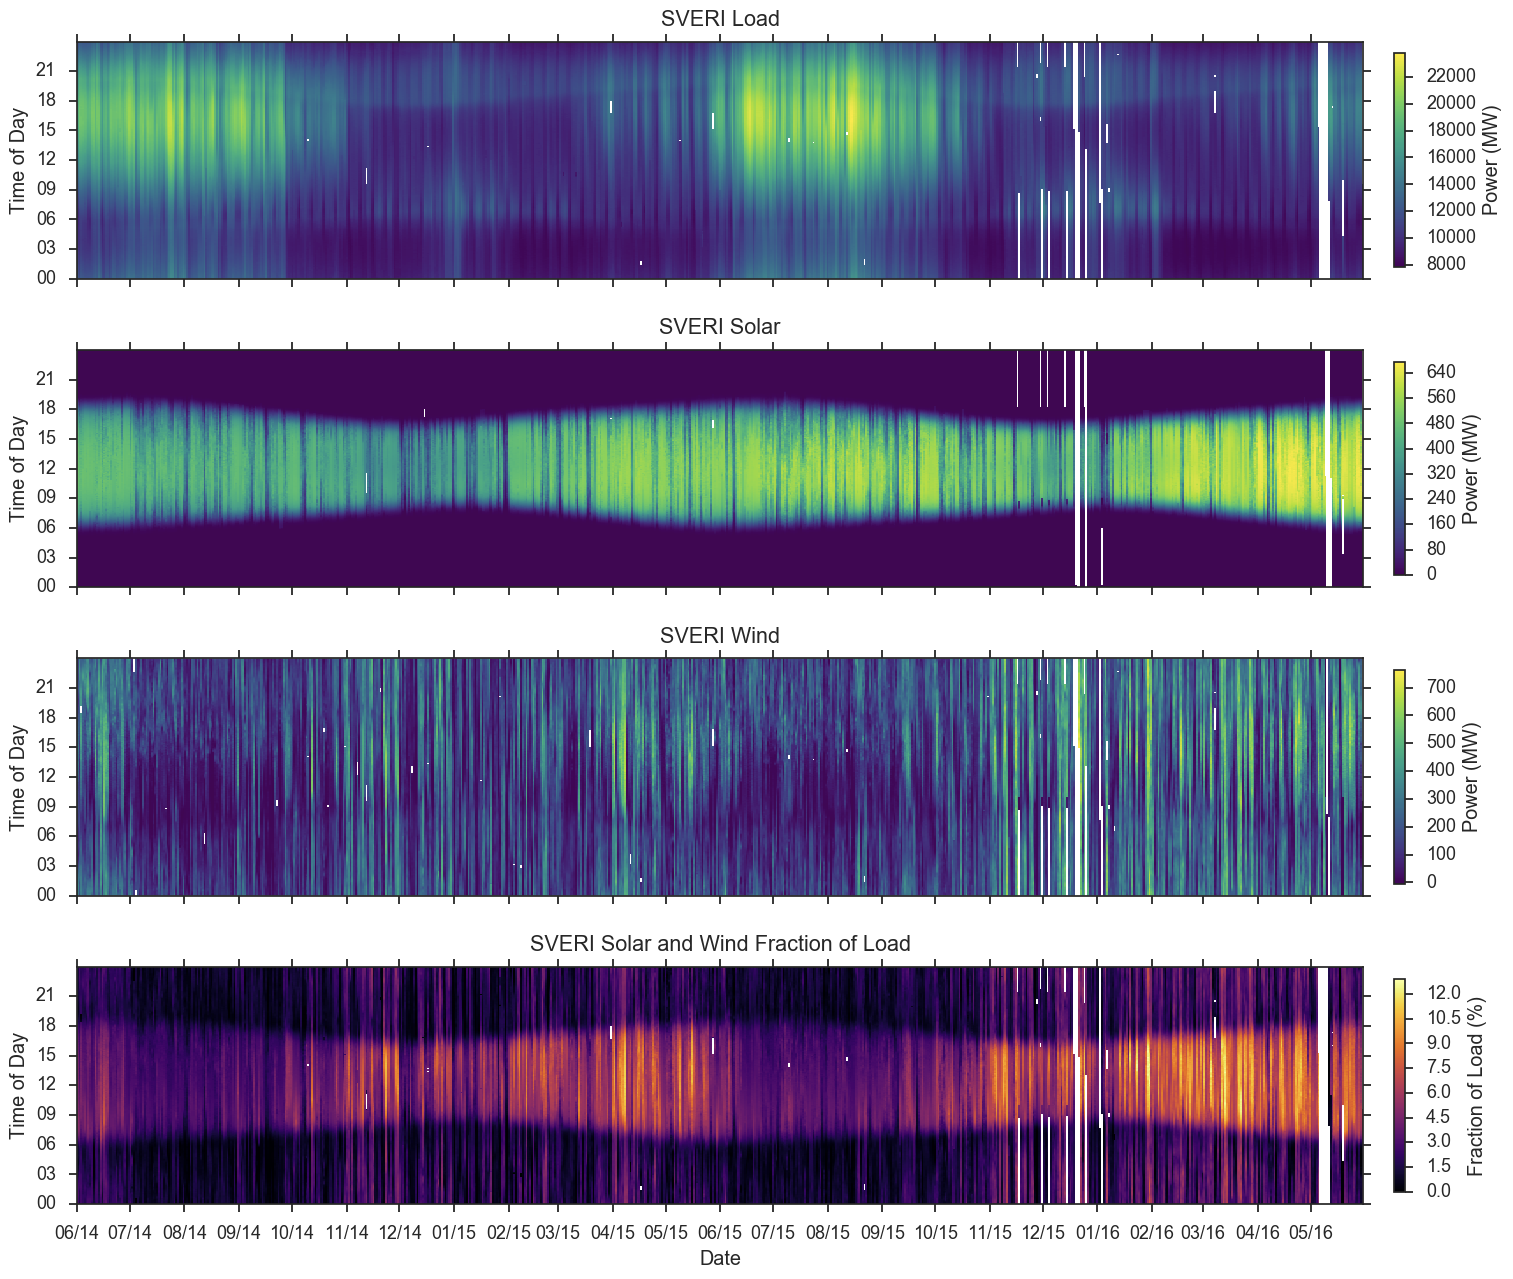
\includegraphics[width=\textwidth]{figs/sveri_heat.png}
\caption[Heatmaps of SVERI load, solar power, wind power, and
renewable load fraction]{Time of day heatmaps of SVERI load, solar
  power generation, wind power generation, and the fraction of load
  served by solar and wind power. The heatmaps were generated with two
  years of data and the white areas indicate missing data. The diurnal
  cycle is clearly seen in the solar data, and can also be found in
  the wind and load. A weekly cycle is also evident in the load. At
  times in the spring when heating and cooling loads are low and their
  is high solar generation, wind and solar power can serve up to 12\%
  of the load.}
\label{fig:sveri_heatmap}
\end{figure}

\begin{figure}[p]
\centering
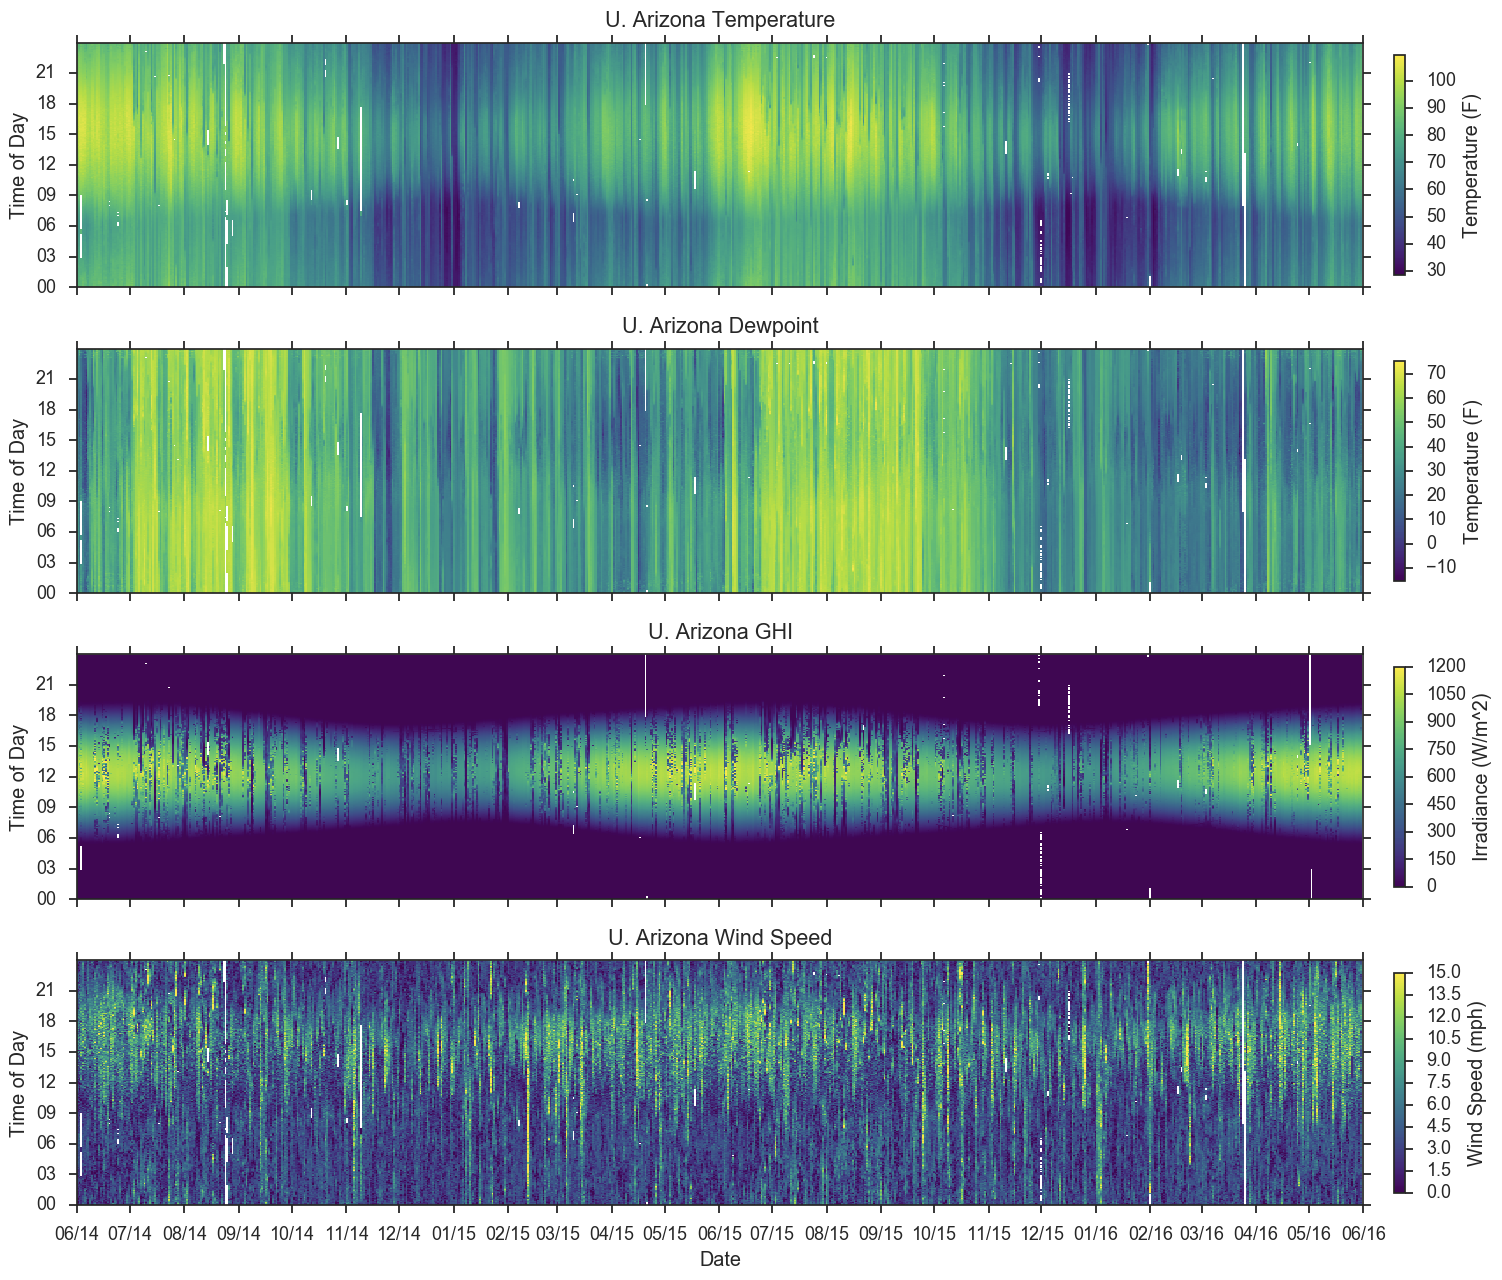
\includegraphics[width=\textwidth]{figs/ua_heat.png}
\caption[Heatmaps of temperature, dewpoint, irradiance, and wind
speed]{Time of day heatmaps for temperature, dewpoint, global
  horizontal irradiance (GHI), and wind speed all measured at the
  University of Arizona in Tucson. Notable features include the many
  clear days evident in the GHI heatmap and the beginning and end of the
  monsoon season (when moisture from the Gulf of California moves into
  Arizona) visible in the dewpoint heatmap.}
\label{fig:ua_heatmap}
\end{figure}

Utilities in Arizona are well on their way to generate 15\% of their
energy from renewable resources by 2025 as required by the Arizona
Renewable Energy Standard and Tariff \citep{azrest}.
As mentioned above, DG solar systems provide a large fraction of the
total renewable energy generation.
One problem utilities encounter with DG systems is that real-time
monitoring is limited.
Since the power generated by these systems can also be consumed on
site, variability in DG power is visible to the utilities as
variability in the load.
Real-time estimates (or nowcasts) and forecasts of this DG variability
will be required for the most accurate load forecasts.

\begin{figure}[h]
\centering
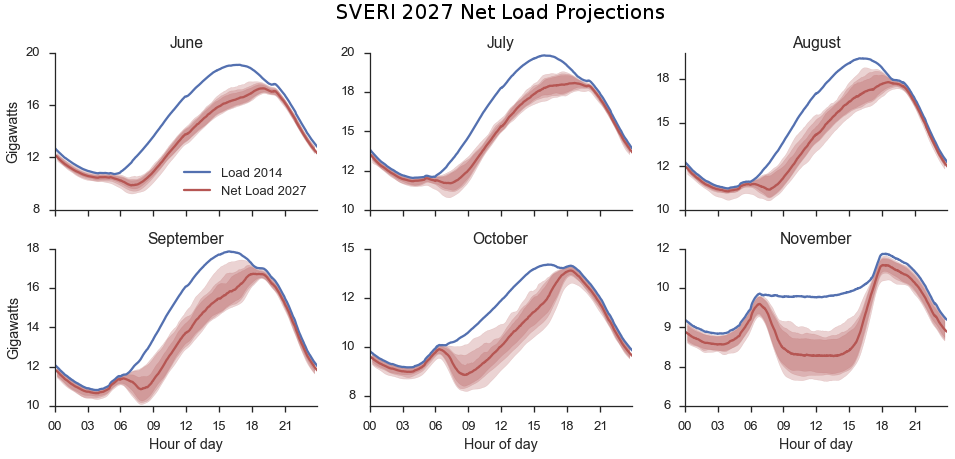
\includegraphics[width=\textwidth]{figs/duckcurves.png}
\caption[Projected SVERI 2027 duck curves]{Net load (total load minus
  wind and solar generation) projections for SVERI in 2027 if
  utilities continue business as usual. The shape of the November net
  load is referred to as a duck curve. Forecasts along with storage
  and other policies will help utilities change how solar and wind
  power are controlled to avoid these multi-GW ramps. Figure
  reproduced from \cite{sveri_report}}
\label{fig:duckcurves}
\end{figure}

Similar to DG, utilities may consider power generated at large solar
and wind power plants to be modifiers of the load instead of power
that is controlled and dispatched.
Utilities are then interested in what they call the net load or the
total load minus the generation from solar and wind power plants.
Based on projections from 2014 SVERI data, we project net load
profiles will resemble those in \cref{fig:duckcurves}.
Notice the large power ramps that occur in the so called duck curve in
November.
Dealing with these 3 GW ramps in only a few hours would cost a great
deal if utilities rely only on the current grid technology.
Using forecasts, utilties can better control large solar and wind
power plants and avoid some of these large ramps.
Other smart grid technologies such as energy storage and time of use
rates will also play a critical role in avoiding these ramps to
maintain the reliability of the grid.

The remainder of this dissertation will focus on the primary input to
solar power plants: sunlight.
We will specifically refer to solar irradiance or the amount of
sunlight in a given area that can perform useful work.

\section{Solar Irradiance Forecasting}
As mentioned above, the solar irradiance that reaches the Earth's
surface is variable.
The first obvious source of variability is the diurnal cycle due to
the movement of the sun through the sky.
The second major source of variability is due to clouds blocking light
from the sun from reaching the surface of the Earth.
Aerosol, dust particles, and water vapor in the atmosphere can also
reduce sunlight, although they often only account for a small
reduction unless there is a dust storm or dense smog.

\begin{figure}[htb]
\centering
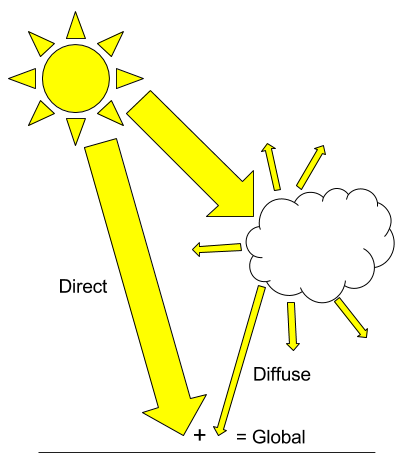
\includegraphics[width=.5\textwidth]{figs/comp_of_irr.png}
\caption{Illustration of direct, diffuse, and global irradiance}
\label{fig:irradiance_components}
\end{figure}

There are three primary classification of the radiation that reaches
the Earth's surface as shown in \cref{fig:irradiance_components}.
The first is the radiation that comes in a straight path directly from
the sun called direct irradiance.
The direct irradiance that strikes the earth at a normal angle is
called the direct normal irradiance (DNI).
Light can also reach the surface by being scattered in the atmosphere
by clouds or aerosols or by features on the surface such as trees and
is referred to as diffuse irradiance.
The total diffuse irradiance that strikes a horizontal surface on the
Earth is referred to as the diffuse horizontal irradiance (DHI).
The sum of the direct and diffuse irradiance is referred to as the
global irradiance, and the total direct and diffused irradiance on a
horizontal surface is called the global horizontal irradiance (GHI).

The majority of solar power plants are non-concentrating systems that
collect both direct and diffuse radiation, thus we will focus on
techniques that forecast GHI.
Furthermore, we are interested in producing forecasts that will,
after being converted to solar power forecasts, be used to maintain
grid reliability and for power market trading similar to
\cite{Kaur2016}.
Thus, we will focus on forecasts that forecast the irradiance now out
to the irradiance a week from now.
Reviews of solar power and irradiance forecasting can be found in
\citep{Inman2013,Antonanzas2016}.

Forecasting techniques are often compared based on the range of
forecast horizons where they outperform a reference forecast as shown
in \cref{fig:fxhoriz}.
This reference can be a persistence forecast that assumes the
irradiance in the future will be the same as it is currently or a
forecast based on climatology.

\begin{figure}[tbh]
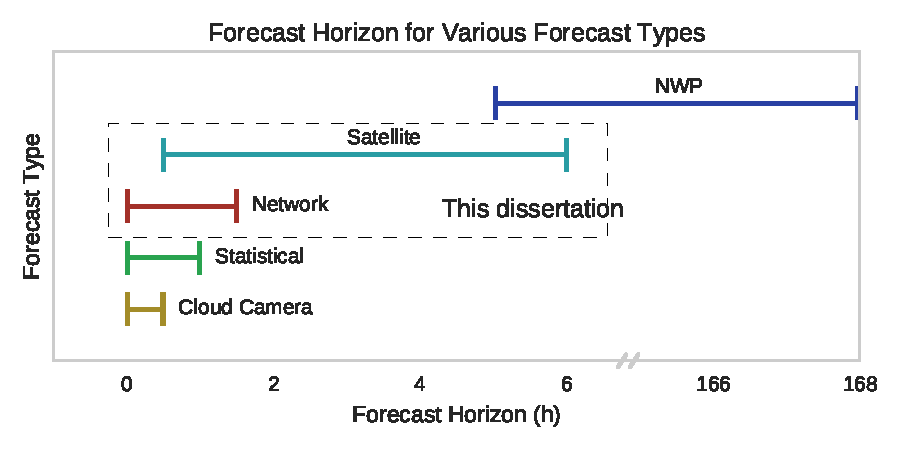
\includegraphics[width=\textwidth]{figs/fxhoriz.pdf}
\caption[Forecast horizon for various forecast types]{The optimal
  forecast horizons for various types of short-term forecasts. This
  dissertation will focus on network and satellite forecasts. NWP
  refers to numerical weather predictions.}
\label{fig:fxhoriz}
\end{figure}

Cloud camera forecasts rely on a camera that is pointed at the sky and
usually includes a wide-angle lens \citep{Urquhart2013}.
Such forecasts use these images to attempt to detect and classify
clouds \citep{Ghonima2012}.
Cloud camera forecasts have been shown to outperform persistence
forecasts at time horizons from under 1 minute to 15 minutes
\citep{Yang2014a}.
These types of forecasts are useful for managing an individual power
plant in near real-time.

Statistical forecasts are those that rely on measured irradiance data,
at least for our purposes.
We include many techniques in this category include auto-regressive
models \citep{Yang2014}, artificial neural networks
\citep{Gutierrez-Corea2016} and other machine learning algorithms
\citep{Pedro2012,Mellit2008}, and the lasso \citep{Yang2015a}.
Persistence forecasts also fall into this category.
These techniques also span a broad range of forecast horizons.
Some provide forecasts for 20 seconds to 10 minutes while others may
produce forecast for many days in advance.

Network forecasts are a type of statistical forecast that will be
studied in depth in this dissertation.
These forecasts depend data from a network of irradiance sensors
deployed over a large area, and they outperform the reference
persistence forecast for time horizons from 1 minute to 2 hours in the
future.
These forecasts are discussed further in \cref{chap:network}.

Satellite forecasts are forecasts that rely on estimates of irradiance
produced from images taken by geostationary satellites.
These estimates can be categorized into semi-empirical and physical models.
Semi-empirical models rely on historical data from the satellite and
ground sensors to find the function that translates from satellite
image pixel to observed irradiance \citep{Perez2013a}.
Physical models try to use the satellite images to infer properties
about the clouds which are then used in a radiative transfer model to
predict the sunlight that reaches the surface \citep{Miller2013}.
Improvements to these irradiance estimates using groud data and data
assimilation will be explored in \cref{chap:satoi}.

Forecasts that predict irradiance for time horizons greater than a few
hours and up to about a week rely on numerical weather predictions
(NWP).
These are dynamic models of the atmosphere that must parameterize
various processes.
One benefit is that NWP forecasts cover a large area.
We produce NWP forecasts using the Weather Research and Forecasting
(WRF) \citep{Skamarock2008} at the University of Arizona with customized
settings for the Southwest \citep{Leuthold}.
Example wind speed and GHI outputs from the UA-WRF model are shown in
\cref{fig:wrf}.
\Cref{chap:future_work} has discussion of possible improvements for
UA-WRF forecasts.
s
\begin{figure}[h]
\subfloat{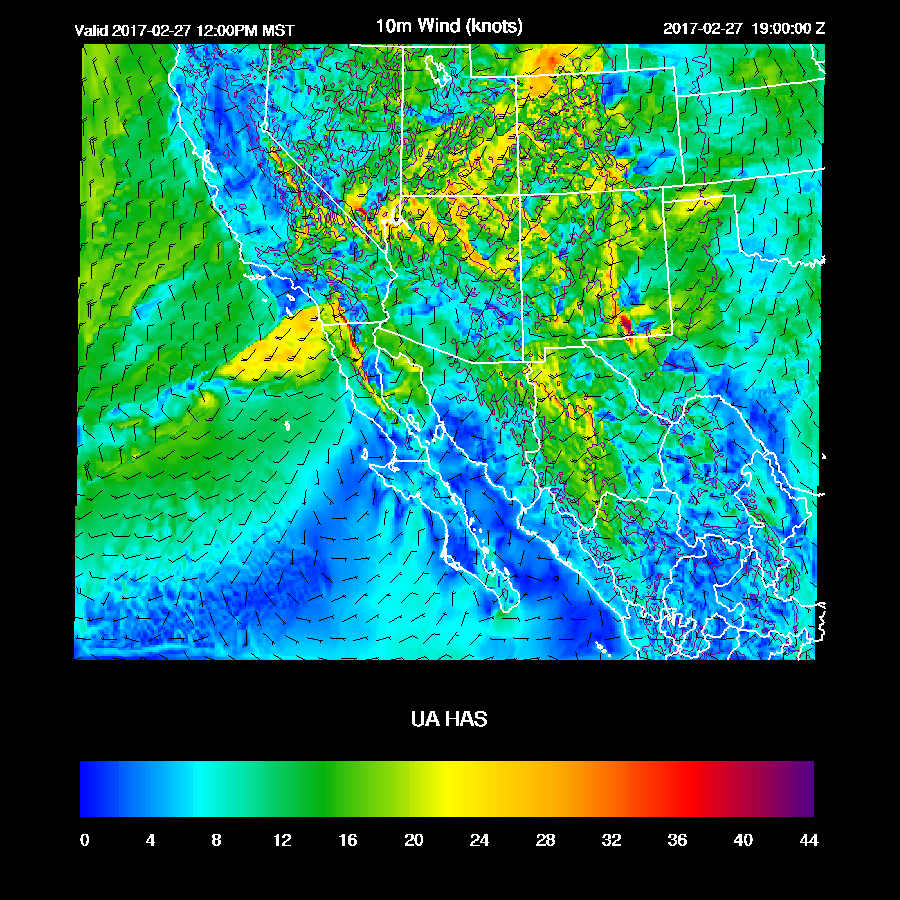
\includegraphics[width=0.5\textwidth]{figs/wrf_wind.png}}
\hspace{-.5em}
\subfloat{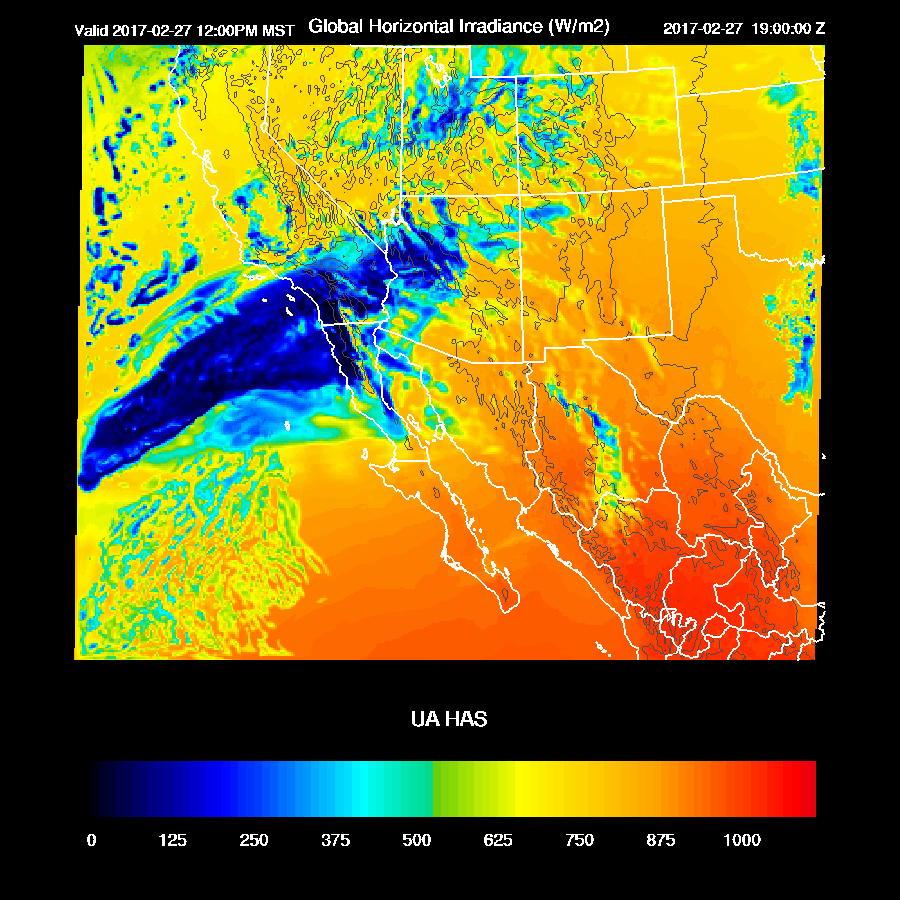
\includegraphics[width=0.5\textwidth]{figs/wrf_ghi.png}}
\caption[Wind speed and GHI output from UA-WRF]{Example wind speed
  near the surface and GHI outputs from the WRF model run at the
  University of Arizona.}
\label{fig:wrf}
\end{figure}

There is also active research in hybrid forecasts that combine
different forecasting techniques to improve forecasts across horizons
\citep{Lu2015}.



\section{This Dissertation in Brief}

\Cref{fig:bullshitplot} shows speculative estimates of
forecast errors as a function of forecast horizon created near the
start of this dissertation work.
This dissertation works to analyze forecasting methods and measure
their errors as a function of forecast horizon in order to
produce the best forecasts of solar irradiance in the Southwest.
\Cref{fig:newshitplot} shows the culmination of this work.

\begin{figure}[htbp]
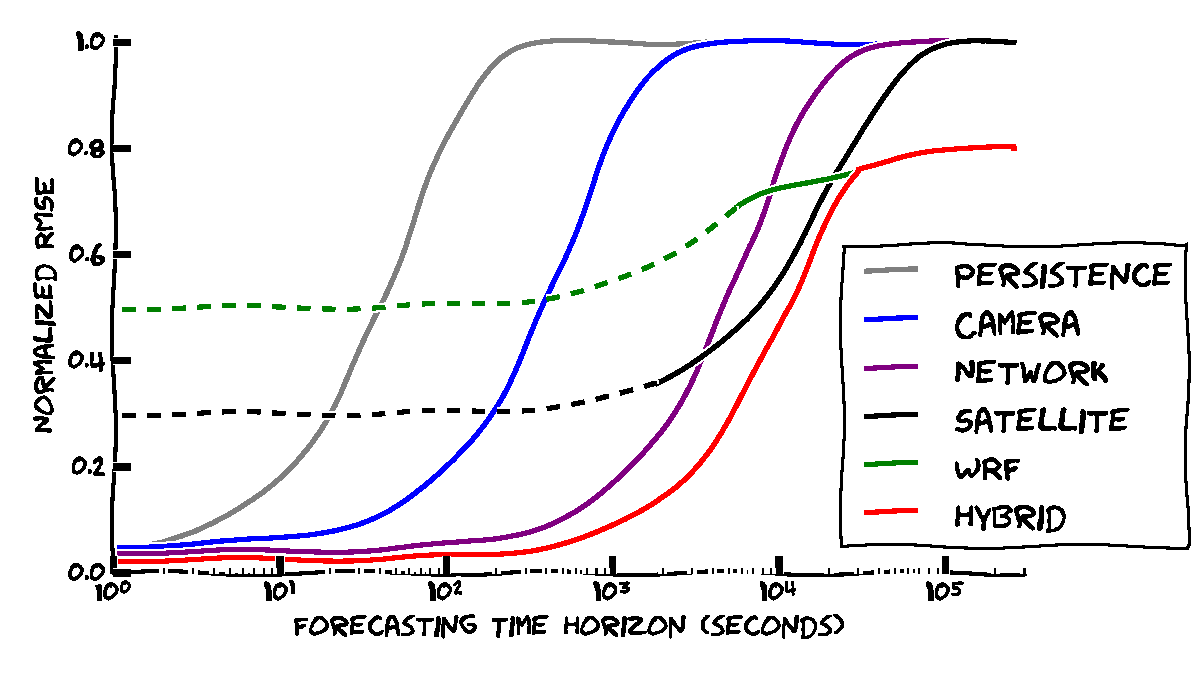
\includegraphics[width=\textwidth]{figs/bullshit.pdf}
\caption[Speculative errors for various forecasting
techniques]{Speculative root mean squared errors (RMSE) for various
  types of forecasts.}
\label{fig:bullshitplot}
\end{figure}

\begin{figure}[htbp]
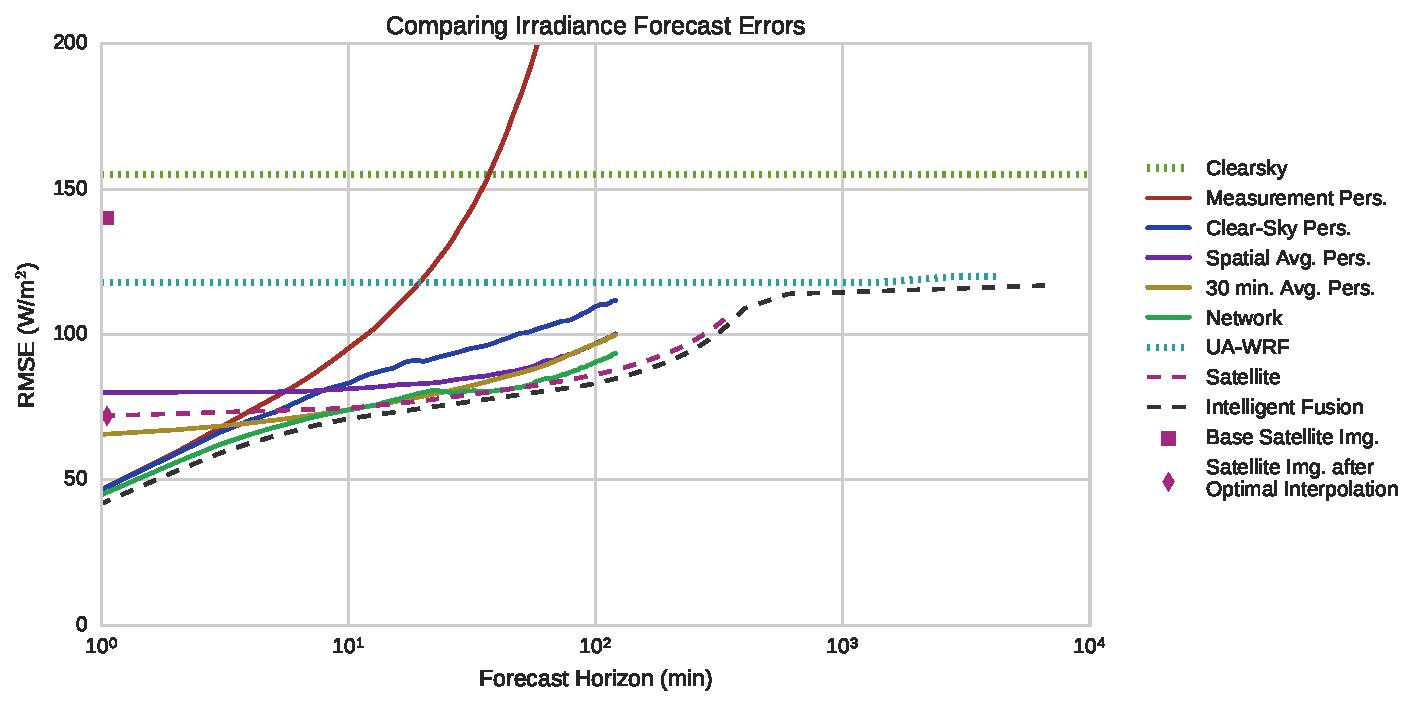
\includegraphics[width=\textwidth]{figs/timehorizon.pdf}
\caption[Irradiance forecast errors across forecast horizons]{A
  comparison of irradiance forecast root-mean squared errors (RMSE)
  across many time horizons.  Pers.\ refers to persistence, and UA-WRF
  refers to the numerical weather models generated at the UA using the
  Weather Research and Forecasting (WRF) model. The intelligent fusion
  is a theoretical combination of forecasts at diffferent time
  horizons for the best forecast at all horizons.  The solid lines
  (and points) indicate forecasts that will be studied in depth in
  this dissertation. Dotted lines are based on prelimnary analysis,
  but have not been studied in depth.  Dashed lines are forecasting
  techniques that will be studied in future work.  The persistence and
  network forecasts will be discussed in \Cref{chap:network} and the
  satellite image points will be discussed in \Cref{chap:satoi}.}
\label{fig:newshitplot}
\end{figure}

The specific forecasting methods studied in this dissertation rely on
a network of irradiance sensors.
A network with sufficient density and time resolution did not exist in
Tucson at the start of this dissertation work, so we set out to design
and deploy inexensive sensors.
The design and deployment of the network is described in
\cref{chap:sens_net}.
For the period of April to July 2014, we collected data from about 50
custom sensors and rooftop PV systems to use in subsequent studies.
All data was detrended to clear-sky index using the expectation of the
output of each sensor on a clear day.

\begin{figure}[htbp]
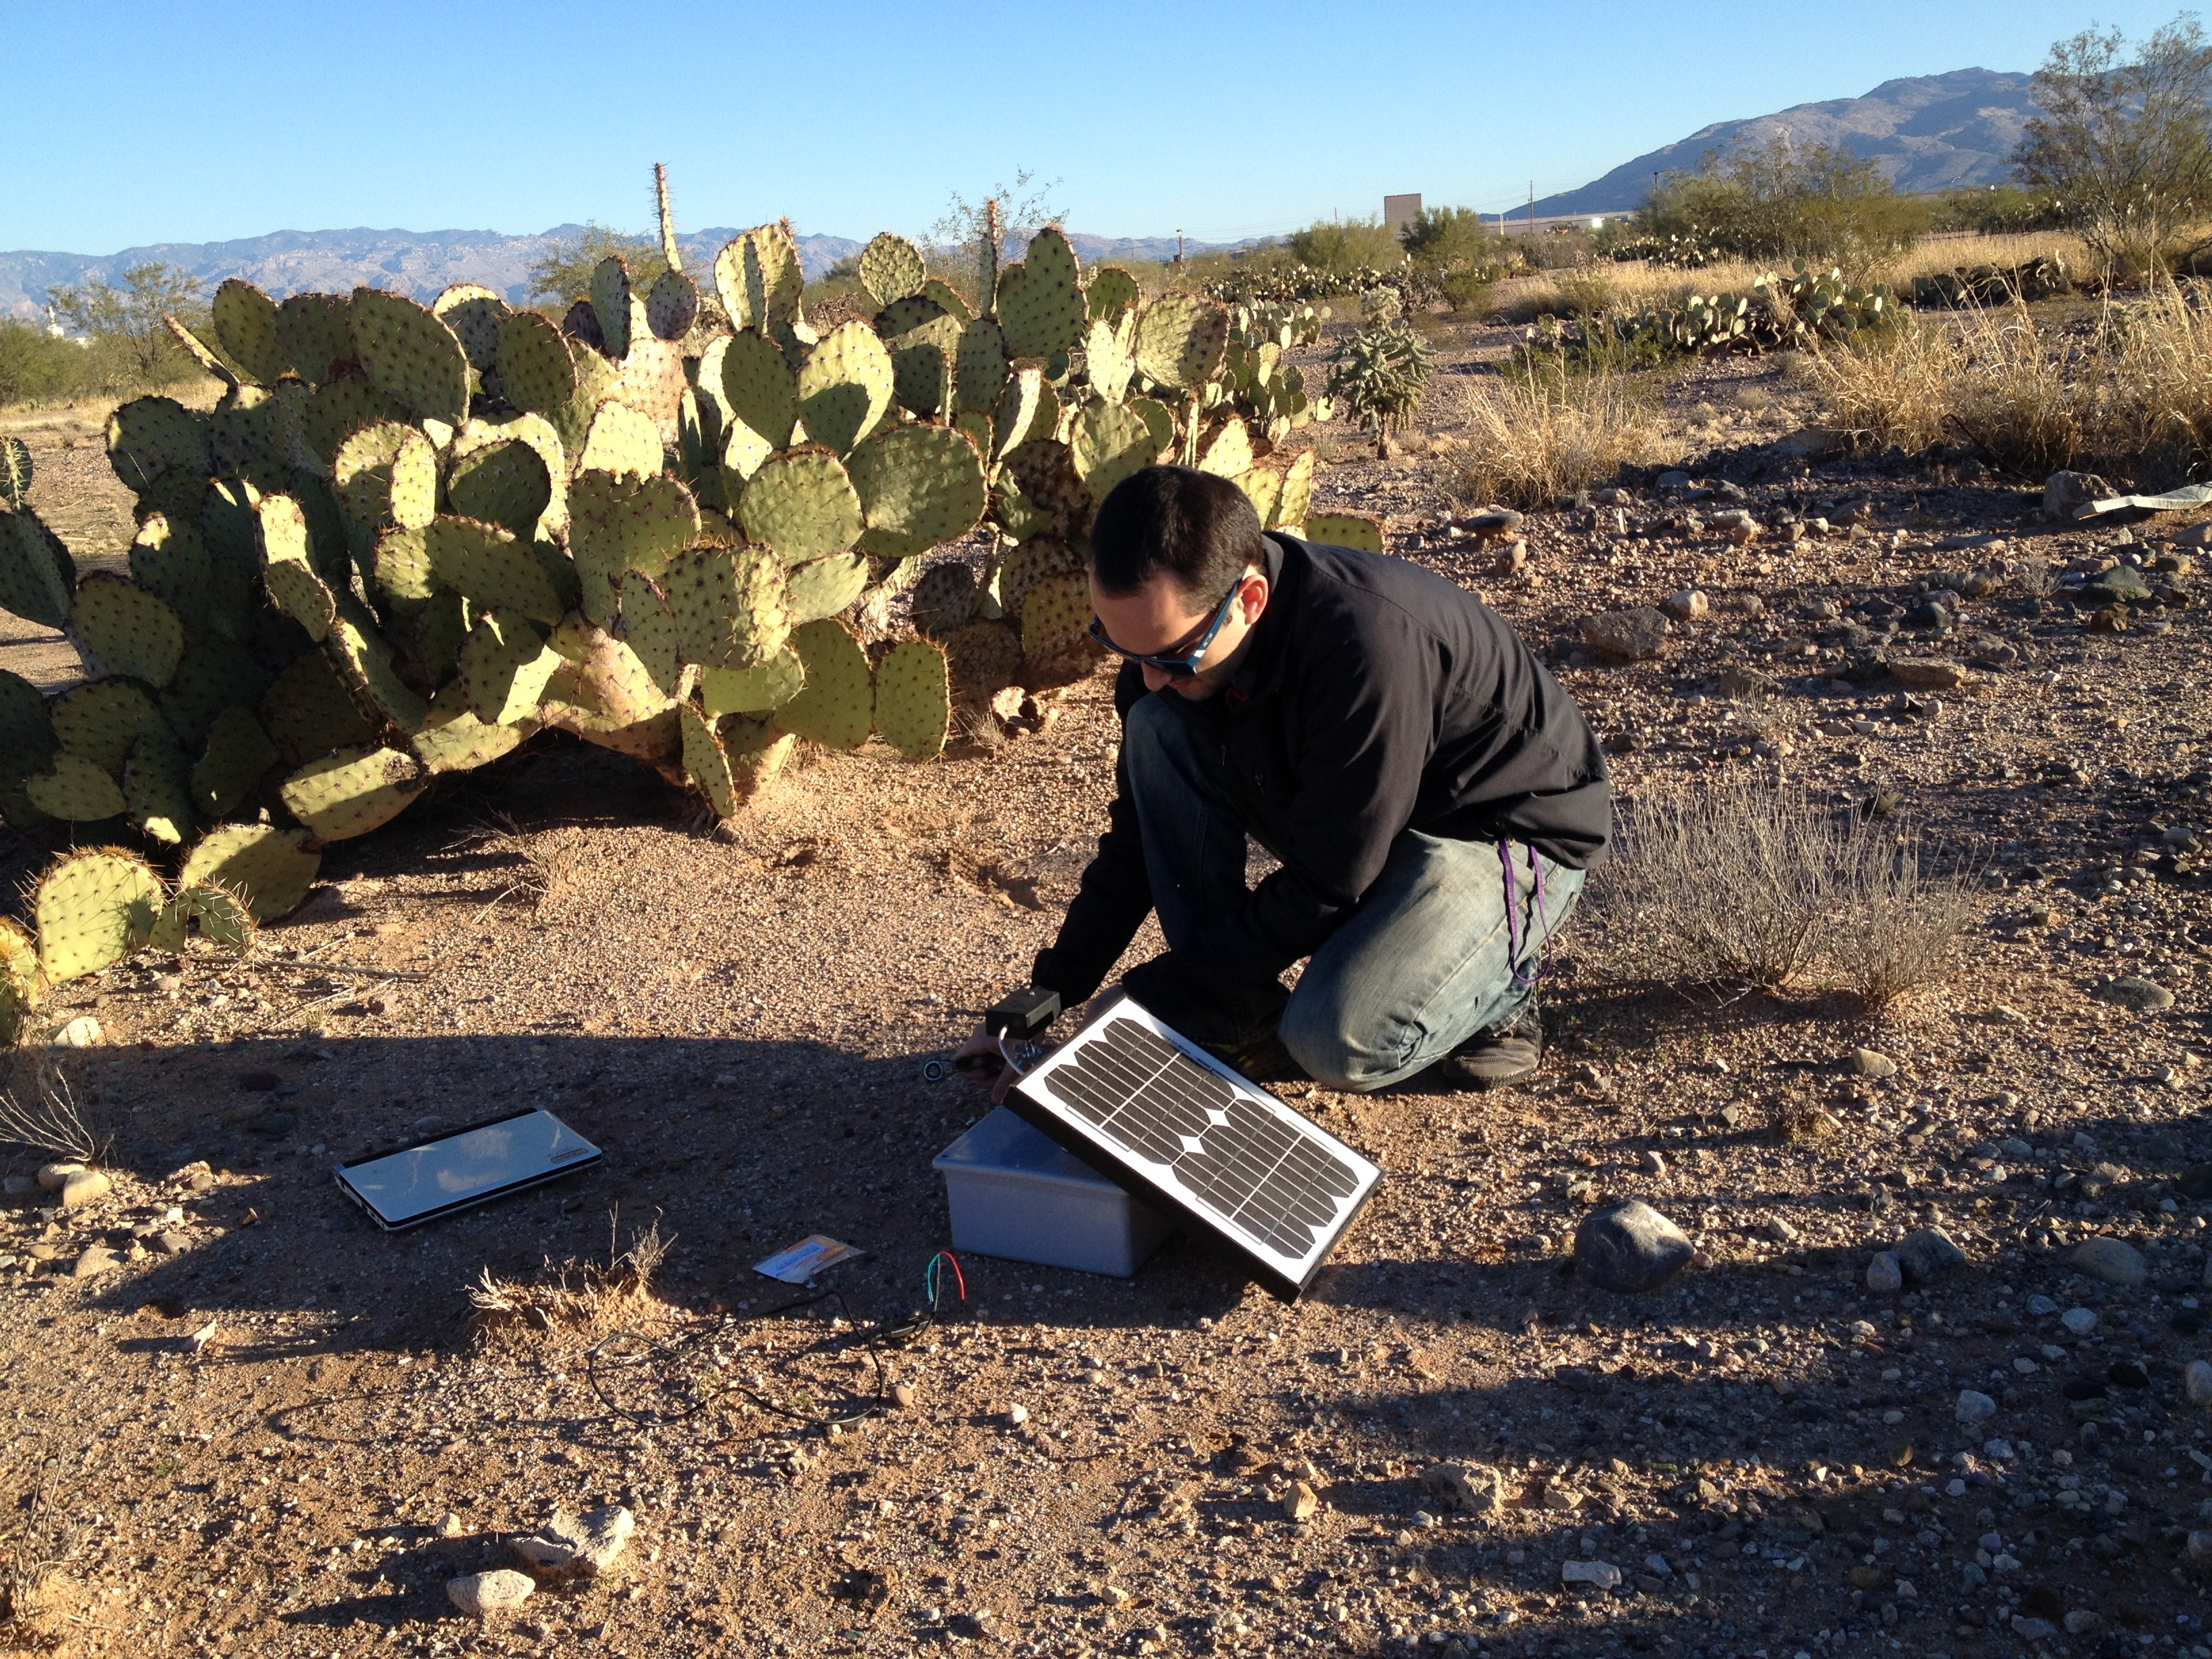
\includegraphics[width=\textwidth]{figs/sensdeploy.jpg}
\caption{Picture of a sensor deployment.}
\end{figure}

With this irradiance network data, the first forecasting methodology
we implemented and analyzed relies only on data from the network as
described in \cref{chap:network}.
This forecast is labeled as network in \cref{fig:newshitplot}.

\begin{figure}[htbp]
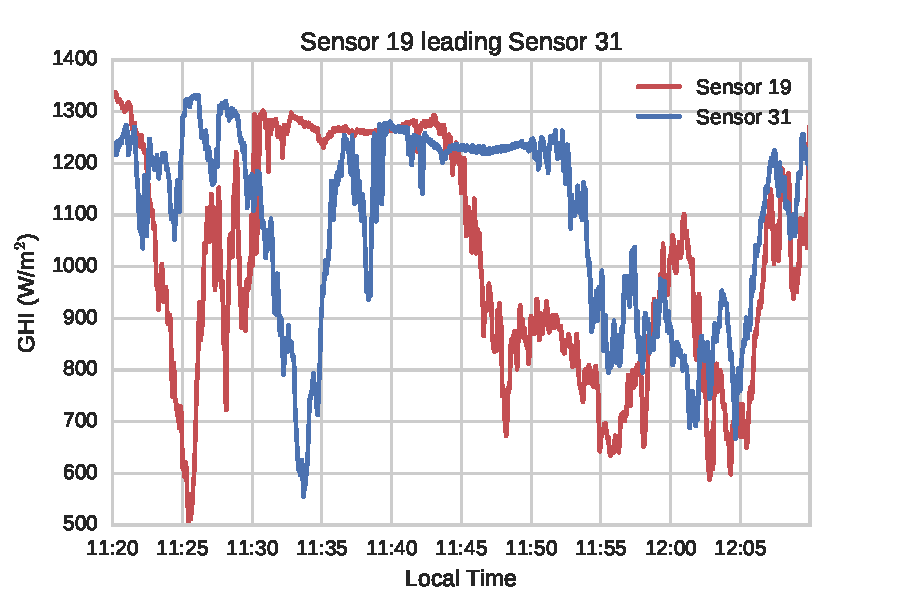
\includegraphics[width=\textwidth]{figs/leading_sens.pdf}
\caption[One sensor predicting the output of another]{An example of
  the output of sensor 19 predicting the output of sensor 31 with a
  roughly 8 minute lead time. This type of correlation is the basis
  for the network forecasts.}
\label{fig:19leading31}
\end{figure}

The basic idea behind this type of forecast is depicted in
\cref{fig:19leading31} where the output of sensor 19 can predict what
the output of sensor 31 will be in 8 minutes.
To generate forecast in practice, we first collect data from the
sensors and interpolate between them to produce a kind of cloud map as
shown in \cref{fig:clearmap}.
Then, using a vector representing the cloud motion, we can move this
map to produce a forecast at any point.
The errors for this type of forecast were studied in depth and a
sample of those errors is shown in \cref{table:network_errors}.
While this method has many paths to improvement, forecasts produced in
this way outperform a persistence forecast by 20\% on average.

\begin{figure}[hbtp]
\centering
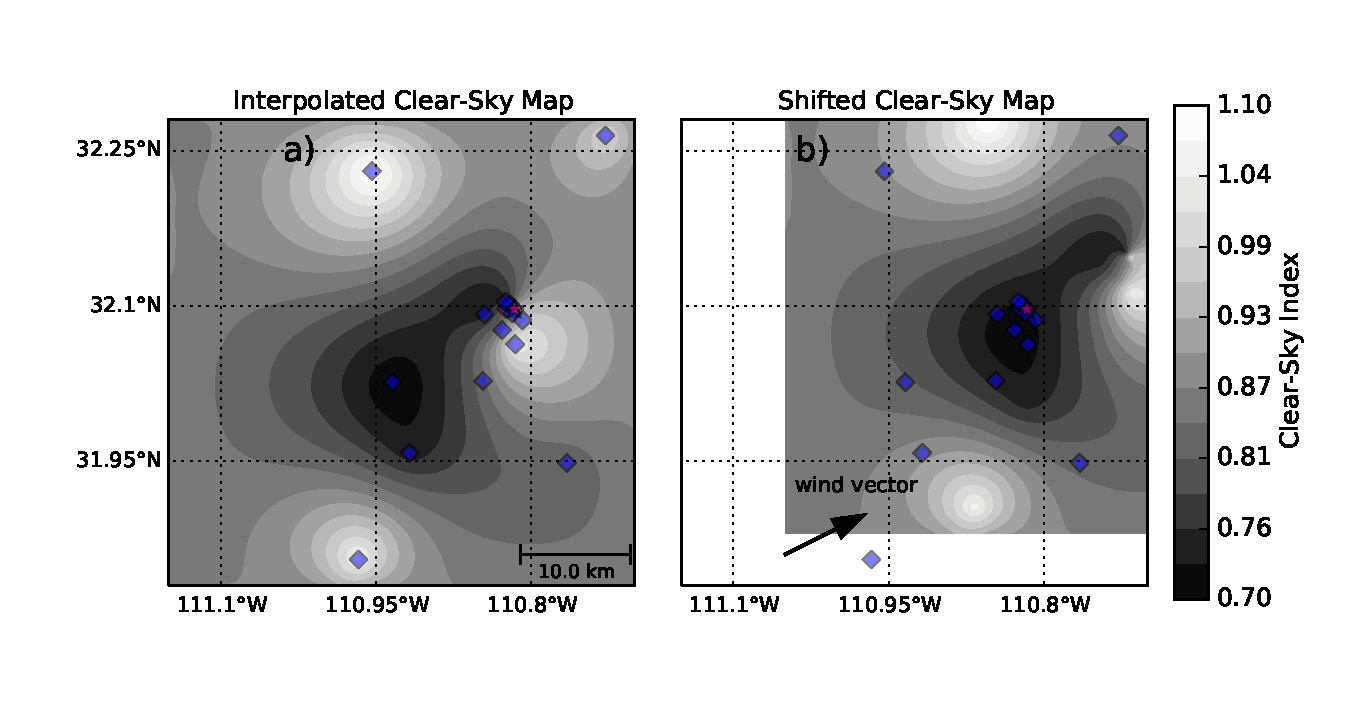
\includegraphics[width=0.96\textwidth]{figs/clearmap.pdf}
\caption[Illustration of the network forecast methodology]{An example
  interpolated map produced from the sensor network data is shown in
  a). Using an estimated cloud motion vector, this map is shifted
  according the the deed forecast horizon as shown in b).}
\label{fig:clearmap}
\end{figure}

\begin{sidewaystable}[p]
\centering
\caption[Error statistics for network forecasts]{
  Summary of error statistics for network forecasts for the 46
  days with clouds. Error statistics were calculated for the entire
  dataset at once. Only forecasts and data with solar zenith angle
  less than $75^\circ$ were used. The mean irradiance was $\bar{y} =
  662 \mbox{ W/m$^2$}$ and the mean clear-sky index was $\bar{k} =
  0.92$.
}
\begin{tabular}{llllllll}
\toprule
FH &  rMAE (\%) &  MAE (W/m$^2$) &  MBE (W/m$^2$) &  rRMSE (\%) &  RMSE (W/m$^2$) &  Avg. skill (\%) \\
\midrule
 1 min  &      4.96 &          30.97 &          -1.44 &      11.90 &           82.55 &           22.96 \\
 3 min  &      7.51 &          48.13 &          -1.39 &      15.89 &          110.46 &           23.09 \\
 5 min  &      9.29 &          59.59 &          -3.91 &      18.67 &          127.06 &           19.65 \\
10 min  &     11.39 &          71.38 &          -8.59 &      22.11 &          141.44 &           18.63 \\
20 min  &     13.23 &          82.39 &         -10.46 &      24.03 &          152.84 &           18.66 \\
30 min  &     13.95 &          86.57 &          -7.52 &      24.49 &          154.15 &           21.21 \\
60 min  &     15.45 &          95.59 &          -6.65 &      26.59 &          160.72 &           21.00 \\
120 min &     17.02 &         106.51 &          -2.01 &      29.20 &          172.45 &           19.58 \\
\bottomrule
\end{tabular}
\label{table:network_errors}
\end{sidewaystable}

\begin{figure}[htbp]
 \centering
 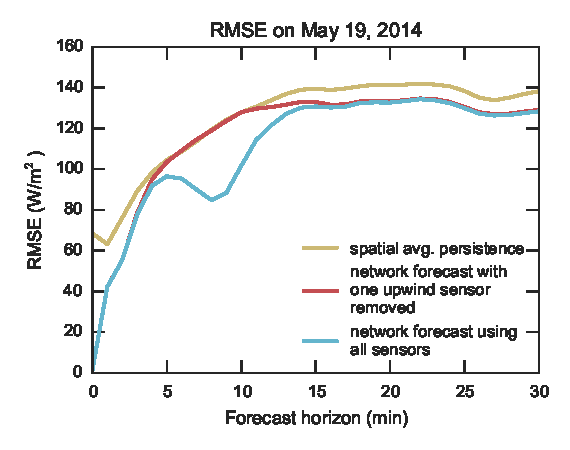
\includegraphics[width=0.9\textwidth]{figs/missing.pdf}
 \caption[Example of a sensor's influence on network forecasts]{RMSE
   vs forecast horizon on May 19, 2014 for network forecasts made with
   all the sensors in the network (blue) and with one upwind sensor
   removed (red), along with a spatially-averaged persistence forecast
   (yellow). The dip at 7 min for the forecast using the full network
   illustrates that properly placed upstream sensors do improve
   forecasts over a simple spatial average.
}
\label{fig:circuitbreak}
\end{figure}

While analyzing this network forecast, we also carefully analyzed
various types of persistence forecasts to understand how the network
forecast works.
\Cref{fig:circuitbreak} shows that network forecasts do incorporate
data from the sensors to improve errors, but at some times the errors
in the network forecast closely resembles the errors of persistence forecasts.
We found that smoother forecasts, or those with lower variance as
compared to the observations, may seem to perform better than
forecasts with higher variance when error metrics are considered in
isolation.
Using the Taylor diagram shown in \cref{fig:taylor}, we show that
network forecasts transition from matching the observation's variance
to essentially becoming an area average persistence forecast after
about 20 minutes.
More details on how to interpret this diagram are described in
\cref{chap:network}.
Thus, we claim that network forecasts are an improvement over spatial
or time averaged persistence forecasts even if they may have similar
RMSE values.

\begin{figure}[htbp]
\centering
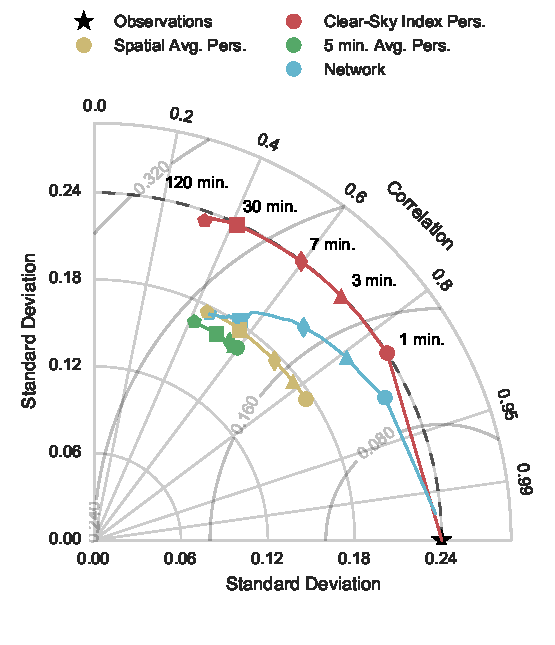
\includegraphics[width=.7\textwidth]{figs/taylor_diagram.pdf}
\caption[Taylor diagram for the network and various persistence
forecasts]{Taylor diagram for clear-sky index persistence (red),
  spatially-averaged persistence (yellow), 5-min time-averaged
  persistence (green), and network (light blue) forecasts for 1 min
  (circle), 3 min (triangle), 7 min (diamond), 30 min (square), and
  120 min (pentagon) forecast horizons. The black dashed line
  indicates the standard deviation of the data. Solid contours around
  the observations point are lines of constant CRMSE. Forecasts for
  clear-sky index were used so all quantities are dimensionless. At
  the 120 min forecast horizon, the spatially-averaged persistence and
  network points overlap. Network forecasts start with a standard
  deviation near that of the measurements, but this decreases at
  longer time horizons as the network forecast begins to resemble
  spatially-averaged persistence.
}
\label{fig:taylor}
\end{figure}

With short-term forecasts covered by the network forecasts, we began
studying forecasts derived from satellite images.
A number of algorithms exist that convert images of the tops of clouds
from geostationary satellites to images of irradiance on the ground.
An example of one such conversion is shown in
\cref{fig:satimage_example}.
Naturally, this conversion from cloud top brightness to the amount of
radiation that passes through clouds is error prone.
We found that these satellite derived irradiance estimates from a
current image (pink square on left axis of \cref{fig:newshitplot}),
before any forecasting is involved, had errors nearly as large as
always assuming the sky were clear.
It is unlikely that producing a forecast from such a nowcast would
reduce errors, so satellite derived forecasts would quickly become
worse than a clear-sky forecast, at least in terms of RMSE.
Thus, in order to produce high quality forcasts from satellite derived
irradiance images, we first improved the satellite derived irradiance
nowcasts.

\begin{figure}[htbp]
\subfloat{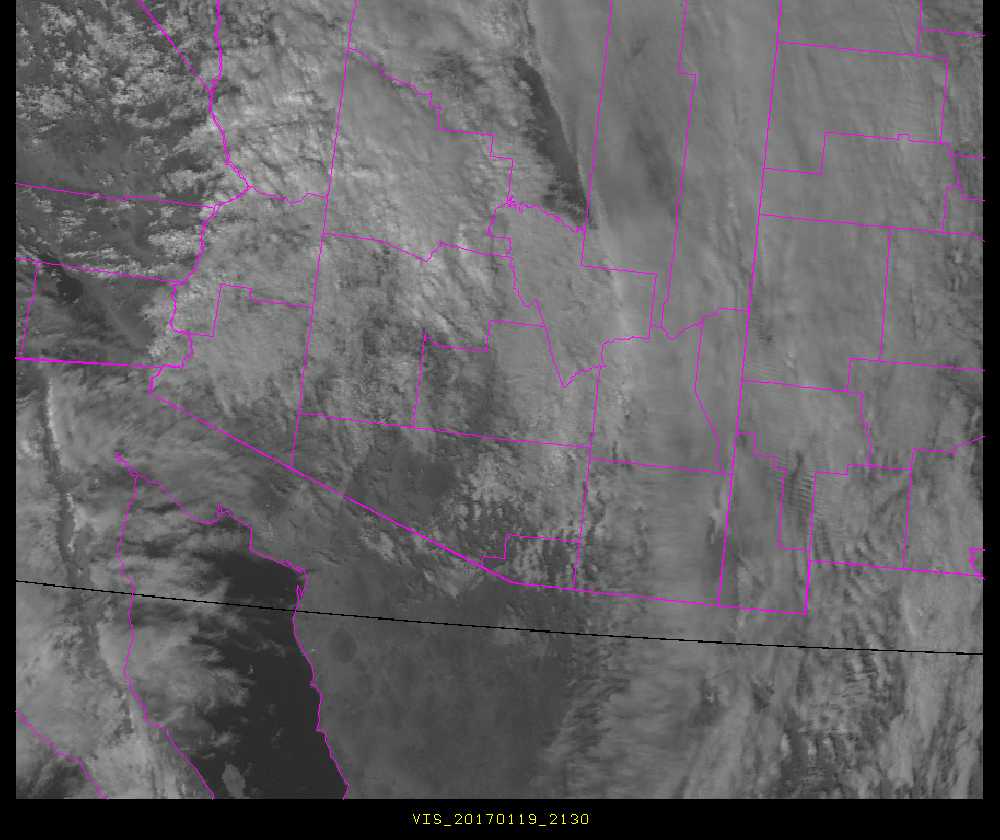
\includegraphics[width=0.5435\textwidth]{figs/rawvis.png}}
\subfloat{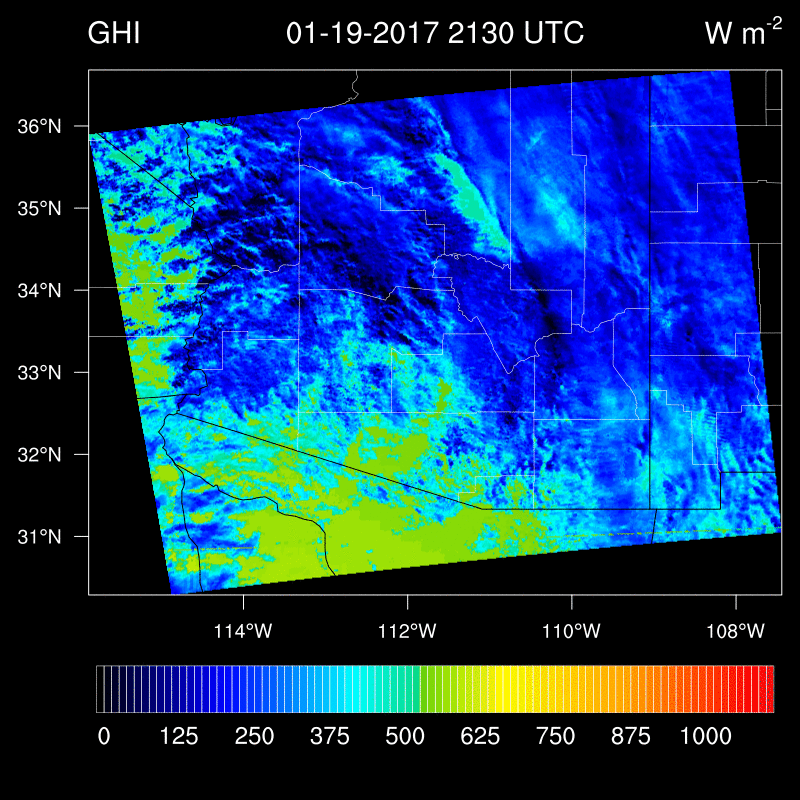
\includegraphics[width=0.4565\textwidth]{figs/satirr.png}}
\caption[Satellite image and irradiance estimate]{A satellite image
  captured by a geostationary satellite (left) and the GHI produced
  from this image (right).}
\label{fig:satimage_example}
\end{figure}

Better satellite derived irradiance nowcasts were generated by again
using data from the irradiance sensor network as described in
\cref{chap:satoi}.
Using a data assimilation method known as optimal interpolation (OI),
we combined the sensor data with the satellite derived irradiance
based on the relative errors between them.
We also parameterized the correlations between pixels in the satellite
images in various ways.
These correlations are responsible for spreading information from the
sensor locations to other locations throughout the image.
An example of improvements using OI is shown in \cref{fig:oi_example}.


\begin{figure}[htbp]
\centering
\captionsetup[subfigure]{labelformat=empty}
\subfloat{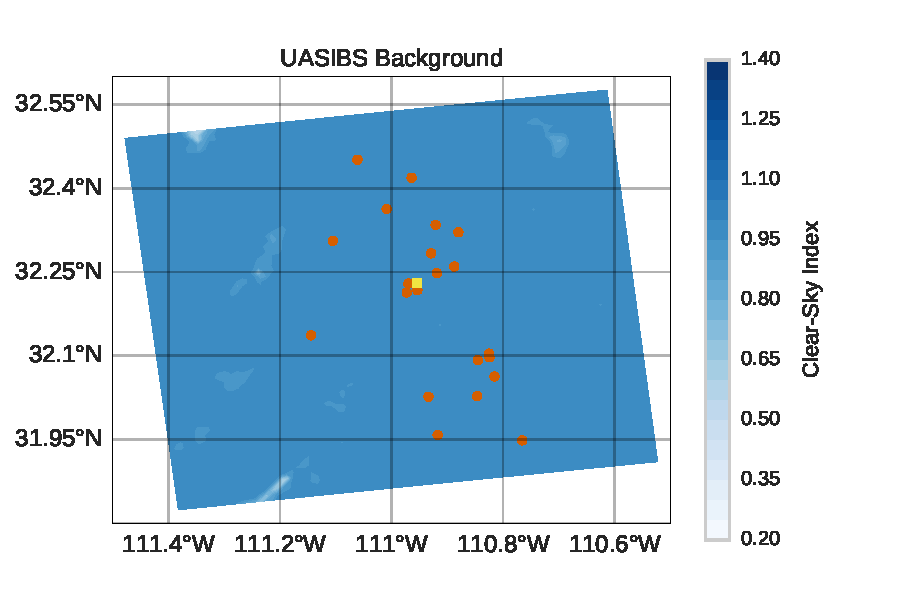
\includegraphics[width=0.5\textwidth]{figs/uasibs_bck_ex.pdf}}
\subfloat{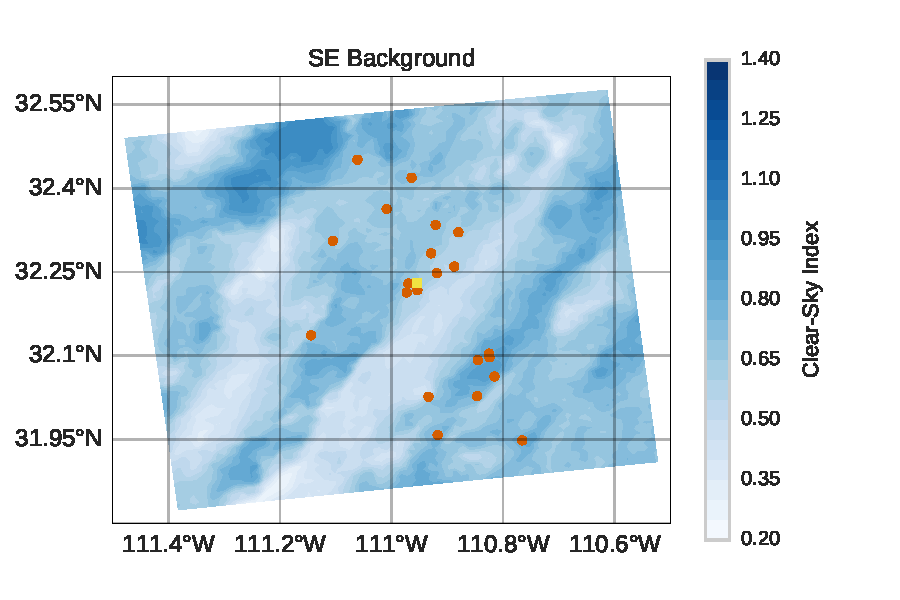
\includegraphics[width=0.5\textwidth]{figs/suny_bck_ex.pdf}}
\vspace{-1em}\\
\subfloat{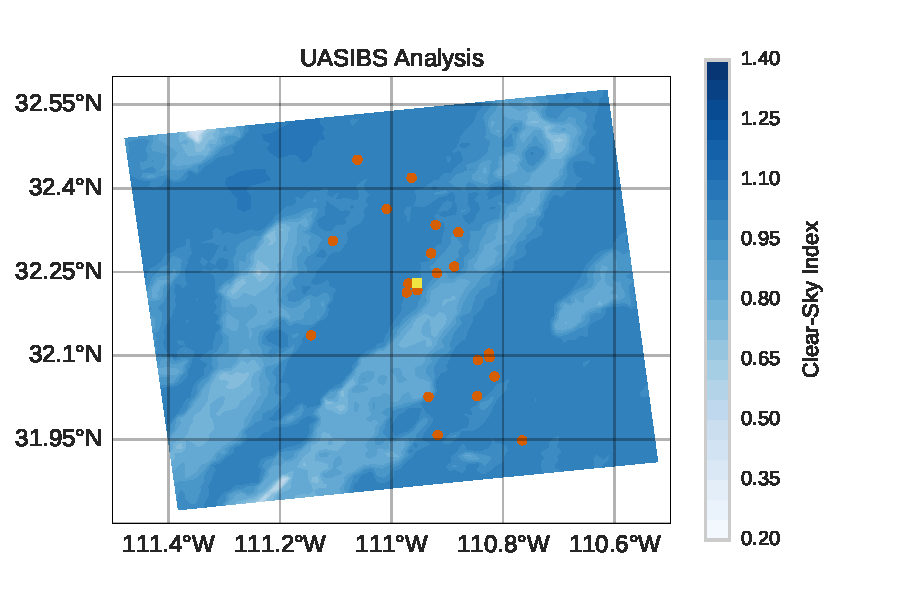
\includegraphics[width=0.5\textwidth]{figs/uasibs_anl_ex.pdf}}
\subfloat{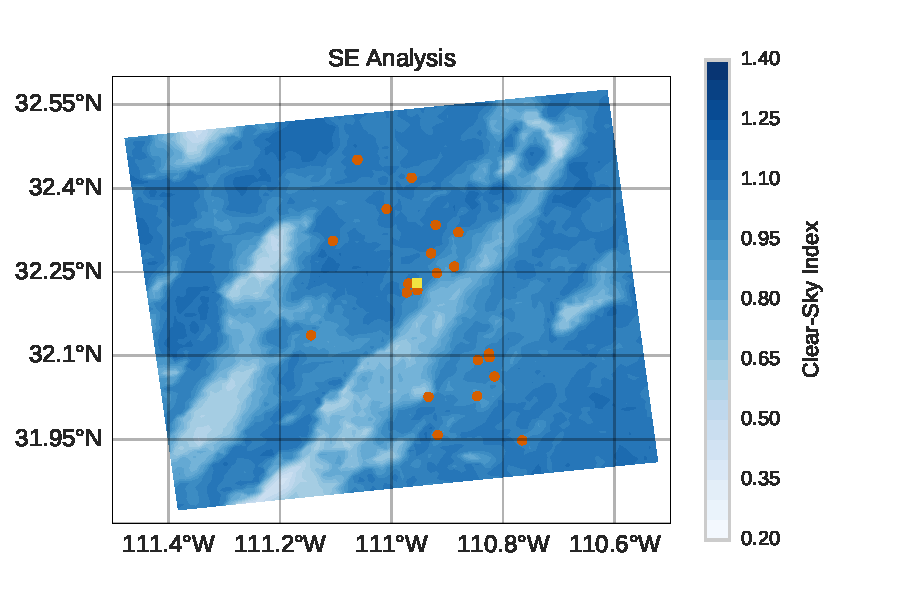
\includegraphics[width=0.5\textwidth]{figs/suny_anl_ex.pdf}}
\caption[Improved satellite irradiance estimates using optimal
interpolation]{Example initial satellite estimate (known as the
  background) (top row) and analysis (bottom row) clear-sky index
  images using a physical (UASIBS, left column) and a semi-empirical
  (SE, right column) satellite image to ground irradiance models Note
  that in this case, UASIBS failed to produce many clouds. OI adds
  clouds to the analysis and also makes the darker, clear areas even
  more clear.  In this case, the SE model overproduces clouds. OI
  reduces the cloud amount while keeping clouds in suitable
  locations.}
\label{fig:oi_example}
\end{figure}

\begin{table}[htbp]
  \caption[Optimal interpolation error metrics]{
    Error statistics for the NREL MIDC sensor on the University
    of Arizona campus. Background refers to the initial satellite
    estimate and the analysis is the result of OI. UASIBS and SE are
    two different satellite image to irradiance models.
    The analysis was computed with only the MIDC
    sensor withheld and averaged over the verification data set, and
    cloudiness covariance was used. Both the
    UASIBS and SE models show improvements and have a similar
    analysis RMSE\@. Units are W/m$^2$.}
\label{table:satoi}
\vspace{0.5em}
\input{figs/ghi_err_table}
\centering
\end{table}


We found significant improvements using this method after various
complicating factors such as misalignment in the satellite image
relative to the ground sensors were corrected.
The improved nowcasts RMSE is shown as the pink diamond in
\cref{fig:newshitplot} and in \cref{table:satoi}
We also found that this method to improve satellite irradiance
nowcasts is applicable to a number of satellite to irradiance
algorithms.

To produce forecasts of irradiance in future work, one might use a
forecasting method that relies on only cloud advection.
With a forecasting model in place, optimal interpolation can be
extended to the Kalman filter with constantly incorporates new data
into a forecast while also retaining information about past data.
It is common in numerical weather prediction to use an ensemble of
states to propogate and Kalman filter.
An ensemble in this case also allows for each forecast to have a
different cloud motion field which may improve the final forecasts.

Satellite forecasts have been shown to perform well for forecast
horizons up to 6 hours.
For longer forecast horizons, numerical weather models are likely
needed.
We currently run the Weather Research and Forecasting (WRF) model with
a custom configuration for Arizona.
Improvements in the WRF model may come from assimilating satellite
data, data from the sensor network, or studying WRF ensembles.

Finally, once high-quality forecasts are available for all forecast
horizons, they can be intellgently fused to produce a single forecast
that incorporates the best properties of each forecast methodology.
Utilities and other stakeholders often need these fused forecasts to
make decisions.


%%% Local Variables:ah
%%% mode: latex
%%% TeX-master: "dissertation"
%%% End:
